\documentclass{beamer}
\usepackage{tikz}
\usetikzlibrary{math}
\usetikzlibrary{intersections}

\usepackage{pgfplots}
\usepgfplotslibrary{polar}

%Please read on the commands and options used below (either in the TikZ / PGFPlots manuals, or elsewhere).

\usepackage{filecontents}
% We're defining a file that will be created upon LaTeX compilation.
% Please note that you need to manually delete the file if you make changes,
% as filecontents does not overwrite files (for obvious security reasons).

%Heaton Research
%https://data.heatonresearch.com › data › auto-mpg

\begin{filecontents*}{clenaed_data.csv}
	mpg	horsepower	regression_line
	24.000000	90.000000	24.910375
	29.800000	90.000000	24.910375
	27.000000	90.000000	24.910375
	19.100000	90.000000	24.910375
	19.000000	90.000000	24.910375
	24.300000	90.000000	24.910375
	23.900000	90.000000	24.910375
	20.000000	90.000000	24.910375
	28.000000	90.000000	24.910375
	20.200000	90.000000	24.910375
	27.000000	90.000000	24.910375
	26.000000	90.000000	24.910375
	18.000000	90.000000	24.910375
	28.000000	90.000000	24.910375
	22.500000	90.000000	24.910375
	20.000000	91.000000	24.666913
	28.000000	92.000000	24.425911
	25.800000	92.000000	24.425911
	25.000000	92.000000	24.425911
	24.000000	92.000000	24.425911
	37.000000	92.000000	24.425911
	26.000000	92.000000	24.425911
	26.000000	93.000000	24.187371
	22.000000	94.000000	23.951291
	25.000000	95.000000	23.717673
	20.000000	95.000000	23.717673
	22.000000	95.000000	23.717673
	23.000000	95.000000	23.717673
	18.000000	95.000000	23.717673
	19.000000	95.000000	23.717673
	23.000000	95.000000	23.717673
	21.100000	95.000000	23.717673
	20.500000	95.000000	23.717673
	24.000000	95.000000	23.717673
	17.500000	95.000000	23.717673
	27.500000	95.000000	23.717673
	25.000000	95.000000	23.717673
	24.000000	95.000000	23.717673
	24.000000	96.000000	23.486516
	25.500000	96.000000	23.486516
	32.000000	96.000000	23.486516
	24.000000	97.000000	23.257820
	18.000000	97.000000	23.257820
	27.200000	97.000000	23.257820
	23.000000	97.000000	23.257820
	19.000000	97.000000	23.257820
	24.000000	97.000000	23.257820
	18.000000	97.000000	23.257820
	22.000000	97.000000	23.257820
	23.900000	97.000000	23.257820
	18.500000	98.000000	23.031585
	22.000000	98.000000	23.031585
	18.000000	100.000000	22.586498
	20.500000	100.000000	22.586498
	19.000000	100.000000	22.586498
	20.000000	100.000000	22.586498
	19.000000	100.000000	22.586498
	23.700000	100.000000	22.586498
	19.000000	100.000000	22.586498
	16.000000	100.000000	22.586498
	19.000000	100.000000	22.586498
	32.900000	100.000000	22.586498
	16.000000	100.000000	22.586498
	15.000000	100.000000	22.586498
	18.000000	100.000000	22.586498
	22.000000	100.000000	22.586498
	18.000000	100.000000	22.586498
	17.000000	100.000000	22.586498
	20.000000	100.000000	22.586498
	20.000000	102.000000	22.151255
	20.300000	103.000000	21.937325
	20.500000	105.000000	21.516849
	23.200000	105.000000	21.516849
	19.200000	105.000000	21.516849
	22.000000	105.000000	21.516849
	16.000000	105.000000	21.516849
	18.000000	105.000000	21.516849
	16.000000	105.000000	21.516849
	26.600000	105.000000	21.516849
	27.900000	105.000000	21.516849
	18.000000	105.000000	21.516849
	18.000000	105.000000	21.516849
	20.600000	105.000000	21.516849
	21.000000	107.000000	21.106217
	19.000000	108.000000	20.904593
	22.400000	110.000000	20.508727
	15.000000	110.000000	20.508727
	17.000000	110.000000	20.508727
	20.000000	110.000000	20.508727
	21.000000	110.000000	20.508727
	17.000000	110.000000	20.508727
	17.500000	110.000000	20.508727
	20.600000	110.000000	20.508727
	18.600000	110.000000	20.508727
	25.000000	110.000000	20.508727
	18.500000	110.000000	20.508727
	21.500000	110.000000	20.508727
	19.900000	110.000000	20.508727
	16.000000	110.000000	20.508727
	18.000000	110.000000	20.508727
	23.500000	110.000000	20.508727
	24.000000	110.000000	20.508727
	21.500000	110.000000	20.508727
	22.000000	112.000000	20.122706
	19.000000	112.000000	20.122706
	18.000000	112.000000	20.122706
	26.000000	113.000000	19.933387
	21.500000	115.000000	19.562132
	21.600000	115.000000	19.562132
	26.800000	115.000000	19.562132
	28.800000	115.000000	19.562132
	25.000000	115.000000	19.562132
	25.400000	116.000000	19.380196
	15.500000	120.000000	18.677064
	18.100000	120.000000	18.677064
	16.500000	120.000000	18.677064
	24.200000	120.000000	18.677064
	20.000000	122.000000	18.340264
	17.000000	125.000000	17.853523
	23.000000	125.000000	17.853523
	19.200000	125.000000	17.853523
	13.000000	129.000000	17.238989
	17.600000	129.000000	17.238989
	18.000000	130.000000	17.091508
	17.000000	130.000000	17.091508
	15.000000	130.000000	17.091508
	13.000000	130.000000	17.091508
	13.000000	130.000000	17.091508
	32.700000	132.000000	16.803930
	16.200000	133.000000	16.663832
	18.200000	135.000000	16.391020
	14.000000	137.000000	16.128052
	16.500000	138.000000	16.000260
	20.200000	139.000000	15.874929
	18.100000	139.000000	15.874929
	13.000000	140.000000	15.752059
	19.400000	140.000000	15.752059
	17.500000	140.000000	15.752059
	16.000000	140.000000	15.752059
	17.000000	140.000000	15.752059
	14.000000	140.000000	15.752059
	17.500000	140.000000	15.752059
	15.500000	142.000000	15.513702
	13.000000	145.000000	15.174625
	15.500000	145.000000	15.174625
	19.200000	145.000000	15.174625
	17.500000	145.000000	15.174625
	15.000000	145.000000	15.174625
	13.000000	145.000000	15.174625
	15.000000	145.000000	15.174625
	14.000000	148.000000	14.857697
	16.000000	149.000000	14.756977
	14.000000	150.000000	14.658717
	13.000000	150.000000	14.658717
	15.000000	150.000000	14.658717
	14.000000	150.000000	14.658717
	13.000000	150.000000	14.658717
	16.000000	150.000000	14.658717
	13.000000	150.000000	14.658717
	16.000000	150.000000	14.658717
	18.000000	150.000000	14.658717
	14.000000	150.000000	14.658717
	11.000000	150.000000	14.658717
	15.000000	150.000000	14.658717
	14.000000	150.000000	14.658717
	13.000000	150.000000	14.658717
	17.000000	150.000000	14.658717
	18.500000	150.000000	14.658717
	15.000000	150.000000	14.658717
	15.000000	150.000000	14.658717
	16.000000	150.000000	14.658717
	14.000000	150.000000	14.658717
	15.000000	150.000000	14.658717
	14.000000	150.000000	14.658717
	14.500000	152.000000	14.469582
	14.000000	153.000000	14.378706
	14.000000	153.000000	14.378706
	13.000000	155.000000	14.204337
	16.900000	155.000000	14.204337
	13.000000	158.000000	13.961241
	14.000000	160.000000	13.811483
	12.000000	160.000000	13.811483
	14.000000	165.000000	13.480156
	17.700000	165.000000	13.480156
	15.000000	165.000000	13.480156
	13.000000	165.000000	13.480156
	12.000000	167.000000	13.364853
	15.500000	170.000000	13.210356
	15.000000	170.000000	13.210356
	13.000000	170.000000	13.210356
	13.000000	170.000000	13.210356
	16.000000	170.000000	13.210356
	14.000000	175.000000	13.002083
	13.000000	175.000000	13.002083
	13.000000	175.000000	13.002083
	14.000000	175.000000	13.002083
	13.000000	175.000000	13.002083
	12.000000	180.000000	12.855336
	16.000000	180.000000	12.855336
	16.500000	180.000000	12.855336
	11.000000	180.000000	12.855336
	12.000000	180.000000	12.855336
	15.500000	190.000000	12.746423
	15.000000	190.000000	12.746423
	13.000000	190.000000	12.746423
	9.000000	193.000000	12.761740
	12.000000	198.000000	12.836490
	15.000000	198.000000	12.836490
	10.000000	200.000000	12.883618
	11.000000	208.000000	13.170571
	11.000000	210.000000	13.266919
	14.000000	215.000000	13.550861
	13.000000	215.000000	13.550861
	10.000000	215.000000	13.550861
	14.000000	220.000000	13.896328
	14.000000	225.000000	14.303323
	14.000000	225.000000	14.303323
	12.000000	225.000000	14.303323
	16.000000	230.000000	14.771845
\end{filecontents*}

\begin{document}
	
	\begin{frame}
		\begin{figure}
			\center
			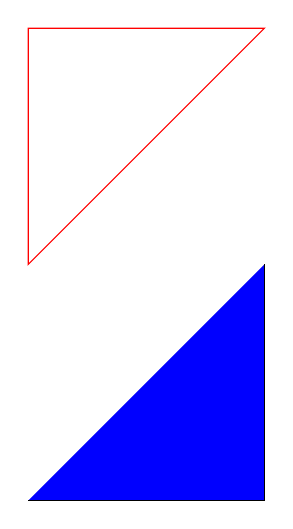
\begin{tikzpicture}[scale=3]
				\draw [fill=blue] (0, 0) -- (1, 0) -- (1, 1);
				\draw [red] (1, 2) -- (0, 2) -- (0, 1) -- cycle;
			\end{tikzpicture}
			\caption{Example 1: Vector drawing in TikZ}
		\end{figure}
	\end{frame}
	
	\begin{frame}
		\begin{figure}
			\center
			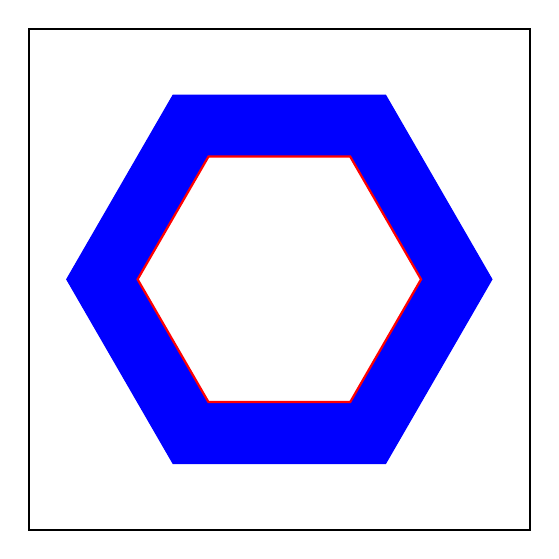
\begin{tikzpicture}[scale=3]
				\draw [black, thick] (45:1.5) -- (135:1.5) -- (225:1.5) -- (315:1.5) -- cycle;
				%
				\fill [blue, even odd rule] 
				( 0:0.6) -- ( 60:0.6) -- (120:0.6) -- (180:0.6) -- (240:0.6) -- (300:0.6) -- cycle
				( 0:0.9) -- ( 60:0.9) -- (120:0.9) -- (180:0.9) -- (240:0.9) -- (300:0.9) -- cycle;
				%
				\draw [red, thick] ( 0:0.6) -- ( 60:0.6) -- (120:0.6) -- (180:0.6) -- (240:0.6) -- (300:0.6) -- cycle;
				\draw [blue] ( 0:0.9) -- ( 60:0.9) -- (120:0.9) -- (180:0.9) -- (240:0.9) -- (300:0.9) -- cycle;
		
			\end{tikzpicture}
			\caption{Task 1: Hexagon drawing}
		\end{figure}
	\end{frame}
	
	
	
	\begin{frame}
		\begin{figure}
			\center
			\begin{tikzpicture}[scale=3]
				% Don't forget ; in \tikzmath. Even after } .
			\tikzmath{%Do not leave empty lines inside tikzmath. Use comments for visual separation
				\xmin = +1000; \xmax = -1000; \ymin = +1000; \ymax = -1000;
				% \tmin = -pi/2;
				% \tmax =  pi/2;
				% \step = 0.05;
				% tikz expects angles in degrees
				\tmin = -90; % -pi / 2 (* 360 / (2*pi))
				\tmax = 90;
				\step = 0.05 * 180 / pi;
				\a = 1;
				\b = 2;
				%{start, ...increment, end}
				for \t in {\tmin + \step, ...\step,\tmax - \step} {
					\x = \a + \b * cos(\t);
					\y = \a * tan(\t) + \b * sin(\t);
					if \x < \xmin then {
						\xmin = \x;
					};
					if \x > \xmax then {
						\xmax = \x;
					};
					if \y < \ymin then {
						\ymin = \y;
					};
					if \y > \ymax then {
						\ymax = \y;
					};
					%
					\x = \a - \b * cos(\t);
					\y = \a * tan(\t) - \b * sin(\t);
					if \x < \xmin then {
						\xmin = \x;
					};
					if \x > \xmax then {
						\xmax = \x;
					};
					if \y < \ymin then {
						\ymin = \y;
					};
					if \y > \ymax then {
						\ymax = \y;
					};
				};
				\xmax = abs(\xmax);
				\xmin = abs(\xmin);
				\ymax = abs(\ymax);
				\ymin = abs(\ymin);
				if \xmin > \xmax then {
					\xmax = \xmin;
				};
				if \ymin > \ymax then {
					\ymax = \ymin;
				};
				%
				\xmprev = (\a + \b * cos(\tmin + \step)) / \xmax;
				\ymprev = (\a * tan(\tmin + \step) + \b * sin(\tmin + \step)) / \ymax;
				for \t in {\tmin + \step, ...\step,\tmax - \step} {
					\xm = (\a + \b * cos(\t)) / \xmax;
					\ym = (\a * tan(\t) + \b * sin(\t)) / \ymax;
					{\draw[blue] (\xmprev, \ymprev) -- (\xm, \ym);};
					\xmprev = \xm;
					\ymprev = \ym;
				};
				\xmprev = (\a - \b * cos(\tmin + \step)) / \xmax;
				\ymprev = (\a * tan(\tmin + \step) - \b * sin(\tmin + \step)) / \ymax;
				for \t in {\tmin + \step, ...\step,\tmax - \step} {
					\xm = (\a - \b * cos(\t)) / \xmax;
					\ym = (\a * tan(\t) - \b * sin(\t)) / \ymax;
					{\draw[blue] (\xmprev, \ymprev) -- (\xm, \ym);};
					\xmprev = \xm;
					\ymprev = \ym;
				};
			}
		\end{tikzpicture}
		\caption{Example 2.1: Nicomedes' Conchoid}
	\end{figure}
\end{frame}

\begin{frame}
	\begin{figure}
		\center
		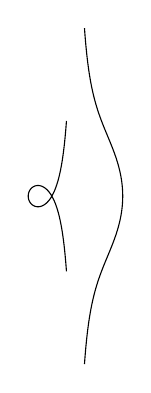
\begin{tikzpicture}
			\def\a{1}
			\def\b{2}
			% {-90+1} so we don't divide by 0. The other +10 are so that we
			% get the picture we want. See the next tikzpicture for a (worse) variant.
			\draw[scale=0.3,domain={-90+11}:{90-11},smooth,variable=\t,samples=180] plot ({\a + \b * cos(\t)}, {\a * tan(\t) + \b * sin(\t)});
			\draw[scale=0.3,domain={-90+11}:{90-11},smooth,variable=\t,samples=180] plot ({\a - \b * cos(\t)}, {\a * tan(\t) - \b * sin(\t)});
		\end{tikzpicture} \hfill
		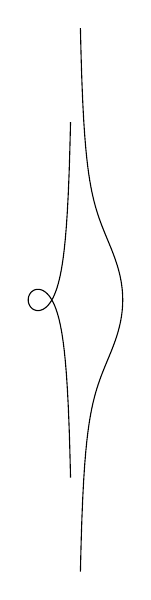
\begin{tikzpicture}
			\def\a{1}
			\def\b{2}
			\draw[scale=0.3,domain={-90+6}:{90-6},smooth,variable=\t,samples=180] plot ({\a + \b * cos(\t)}, {\a * tan(\t) + \b * sin(\t)});
			\draw[scale=0.3,domain={-90+6}:{90-6},smooth,variable=\t,samples=180] plot 	({\a - \b * cos(\t)}, {\a * tan(\t) - \b * sin(\t)});
		\end{tikzpicture}
		\caption{Example 2.2: Nicomedes' Conchoid, auto-plot}
	\end{figure}
\end{frame}


\begin{frame}
	\begin{figure}
		\center
		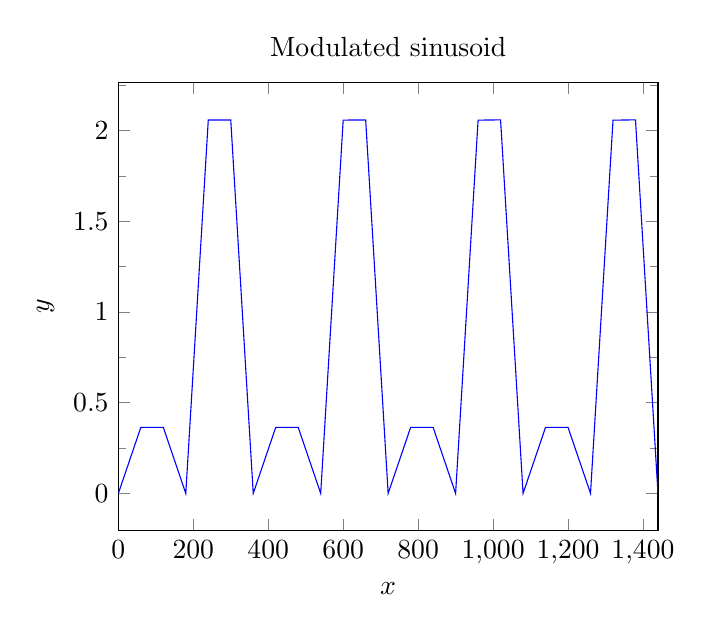
\begin{tikzpicture}
			\begin{axis}[
				title=Modulated sinusoid,
				xlabel={$x$},
				ylabel={$y$},
				domain={0}:{8 * 180}, %8 * pi
				xmin=0, xmax= {8 * 180}, %the actual limits of the plot
				minor y tick num=1, %how many unlabeled ticks between labeled ticks
				]
				\addplot [blue] {abs(sin(x)) * exp(-sin(x))};
			\end{axis} 
		\end{tikzpicture}
		\caption{Example 2.3: Modulated sinusoid, using PGFPlots. Rough.}
	\end{figure}
\end{frame}

\begin{frame}
	\begin{figure}
		\center
		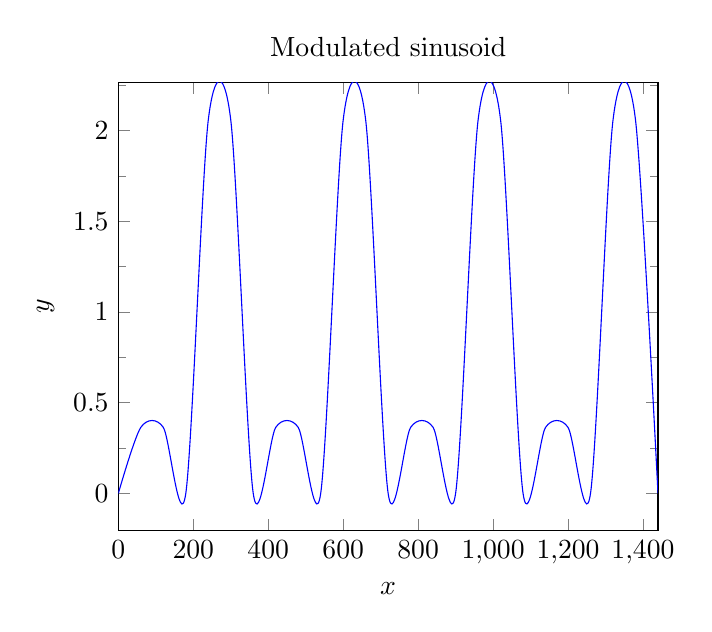
\begin{tikzpicture}
			\begin{axis}[
				title=Modulated sinusoid,
				xlabel={$x$},
				ylabel={$y$},
				domain={0}:{8 * 180}, %8 * pi
				xmin=0, xmax= {8 * 180}, %the actual limits of the plot
				minor y tick num=1, %how many unlabeled ticks between labeled ticks
				smooth,
				]
				\addplot [blue] {abs(sin(x)) * exp(-sin(x))};
			\end{axis} 
		\end{tikzpicture}
		\caption{Example 2.4: Modulated sinusoid, using PGFPlots. Rough, artificially smoothed.}
	\end{figure}
\end{frame}

\begin{frame}
	\begin{figure}
		\center
		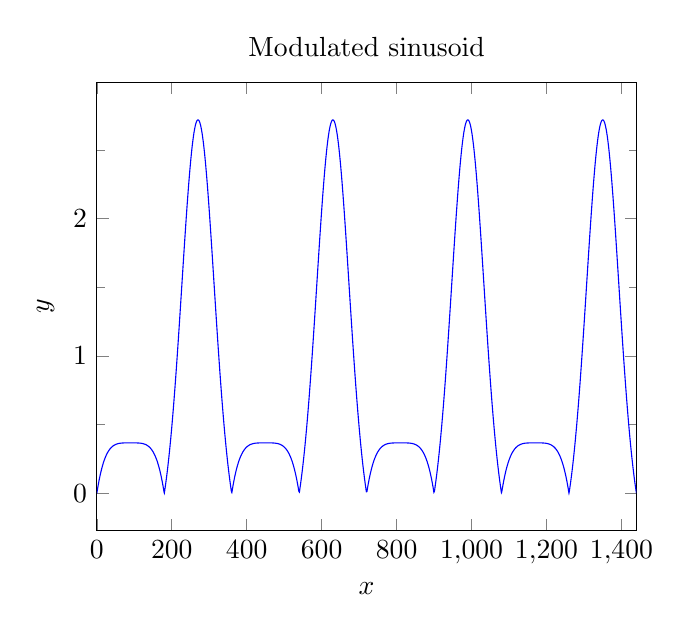
\begin{tikzpicture}
			\begin{axis}[
				title=Modulated sinusoid,
				xlabel={$x$},
				ylabel={$y$},
				domain={0}:{8 * 180}, %8 * pi
				xmin=0, xmax= {8 * 180}, %the actual limits of the plot
				minor y tick num=1, %how many unlabeled ticks between labeled ticks
				smooth,
				samples=1000,
				]
				\addplot [blue] {abs(sin(x)) * exp(-sin(x))};
			\end{axis} 
		\end{tikzpicture}
		
		\caption{Example 2.5: Modulated sinusoid, using PGFPlots. Better sampled.}
	\end{figure}
\end{frame}

\begin{frame}
	\begin{figure}
		\center
		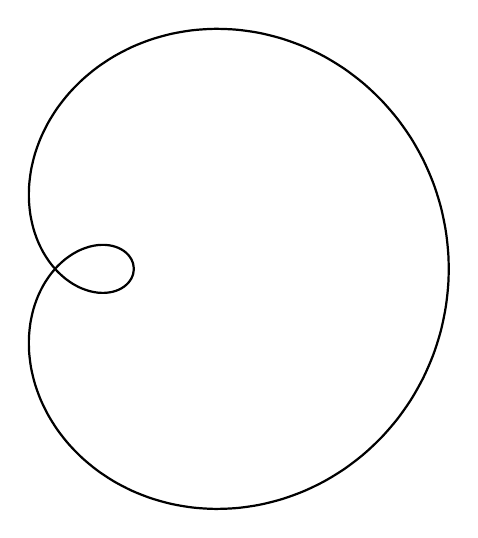
\begin{tikzpicture}
			\def\a{0.3}
			\def\b{0.2}
			%Limitele intervalului
			\def\minus_pi{-180}
			\def\pi{180}
			\draw[black, thick, scale=5,domain=\minus_pi:\pi,smooth,variable=\t,samples=100] 
			plot ({2*(\a*cos(\t) + \b)*cos(\t)}, {2*(\a*cos(\t) + \b)*sin(\t)});
		\end{tikzpicture}
		\caption{Task 2: Circle Concoid}
	\end{figure}
\end{frame}

\begin{frame}
	\begin{figure}
		\center
		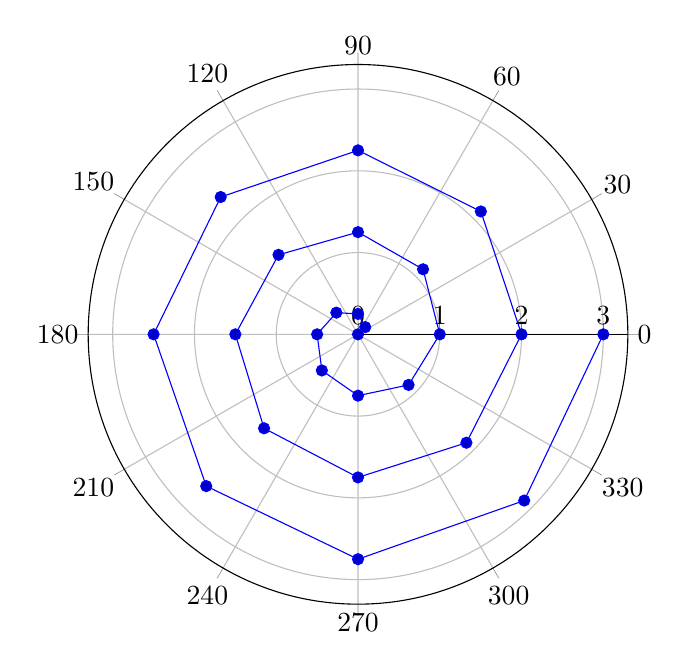
\begin{tikzpicture}
			\begin{polaraxis}
				%try \addplot, notice the difference
				\addplot+ [domain=0:3] (360*x,x); % (angle,radius)
			\end{polaraxis} 
		\end{tikzpicture}
		\caption{Example 3: Polar plotting}
	\end{figure}
\end{frame}

\begin{frame}
	\begin{figure}
		\center
		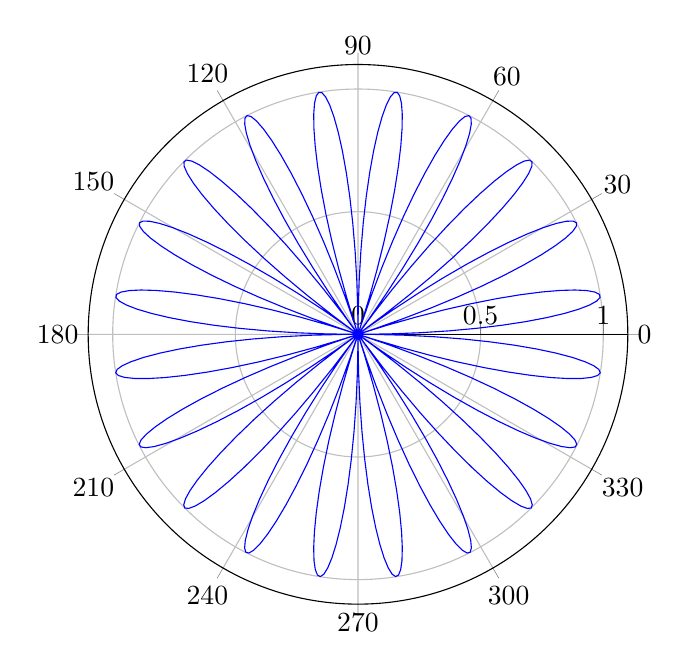
\begin{tikzpicture}
			\begin{polaraxis}[
				yticklabels={-0.5,0,0.5,1}, ytick distance=0.5
				]
				\addplot+[mark=none,domain=0:360,samples=500] 
				{2*(sin(5*x)*cos(5*x))}; 
			\end{polaraxis}
		\end{tikzpicture}
		\caption{Task 3: Polar plotting}
	\end{figure}
\end{frame}

\begin{frame}
	\begin{figure}
		\center
		\begin{tikzpicture}
			\begin{axis} [
				title=Miles per gallon,
				xlabel=hosepower,
				ylabel=mpg,
				]
				\addplot coordinates {
					(140, 18)
					(140, 17)
					(150, 16)
					(180, 15)
					(220, 14)
				};
				%try removing only marks
				\addplot table [x=horsepower, y=mpg, col sep=comma, only marks] {mpg.csv};
			\end{axis} 
		\end{tikzpicture}
		\caption{Example 4: Plotting datafiles, and coordinates.}
	\end{figure}
\end{frame}

\begin{frame}
	\begin{figure}[h!]
		\center
		\begin{tikzpicture}
			\begin{axis}[
				title={Graficul dintre MPG și Horsepower},
				xlabel={Horsepower},
				ylabel={MPG},
				scatter/classes={a={mark=o,blue}}
				]
				\pgfplotstableread[col sep=comma]{D:\\Facultate\\GPC\\cleaned_data.csv}\loadeddata
				\addplot[only marks, scatter, mark=*, blue] table[x=horsepower, y=mpg] {\loadeddata};
			\end{axis}
		\end{tikzpicture}
		\caption{Task 4: Graficul dintre MPG si Horsepower}
	\end{figure}
\end{frame} 

\begin{frame}
	\begin{figure}
		\center
		\begin{tikzpicture}
			\begin{axis}[
				title={Relatia dintre MPG si Horsepower},
				xlabel={Horsepower},
				ylabel={MPG},
				]
				\pgfplotstableread[col sep=comma]{D:\\Facultate\\GPC\\cleaned_data.csv}\loadeddata
				\addplot[only marks, mark=*, blue] table[x=horsepower, y=mpg] {\loadeddata};
				\addplot[thick, red] table[x=horsepower, y=regression_line] {\loadeddata};
			\end{axis}
		\end{tikzpicture}
		\caption{Task 5: Graficul MPG si Horsepower cu regresie}
	\end{figure}
\end{frame}

%sorted_indices = np.argsort(horsepower)
%horsepower = horsepower[sorted_indices]
%mpg = mpg[sorted_indices]
%
%
%coef = np.polyfit(horsepower, mpg, deg=2)
%print(coef)
%poly_eq = np.poly1d(coef)
%regression_line = poly_eq(horsepower)
%
%(regression_line)
%
%np.savetxt("cleaned_data.csv", np.column_stack((mpg, horsepower,regression_line)), delimiter=",", %header="mpg,horsepower,regression_line", comments="", fmt="%f")

\end{document}
